\savestack{\nnfruitclassexample}{\begin{tikzpicture}[scale=1,transform shape]
	\draw (0, 0) rectangle (7, 2);
	\draw (3.5,1) node[text width=3.5cm] {Neural network with $L-1$ hidden layers};
	\draw[thick,->] (1,-1) -- (1,0);
	\draw[thick,->] (2,-1) -- (2,0);
	\draw[thick,->] (3,-1) -- (3,0);
	\draw[thick,->] (4,-1) -- (4,0);
	\draw[thick,->] (5,-1) -- (5,0);
	\draw[thick,->] (6,-1) -- (6,0);
	\draw[thick,->] (1.4,2) -- (1.4,3) node[above] {\footnotesize Apple};
	\draw[thick,->] (2.8,2) -- (2.8,3) node[above] {\footnotesize Mango};
	\draw[thick,->] (4.2,2) -- (4.2,3) node[above] {\footnotesize Orange};
	\draw[thick,->] (5.6,2) -- (5.6,3) node[above] {\footnotesize Banana};
	\draw (3.1,3.5) node[above] {\large $y = \left[ 1 \hspace{1.2cm} 0 \hspace{1.2cm} 0 \hspace{1.2cm} 0 \right]$};
	\node[inner sep=0pt] (russell) at (3.5,-2)
	{
\includegraphics[width=.25\textwidth]{apple.jpg}};
\end{tikzpicture}
}
\savestack{\nnimdbexample}{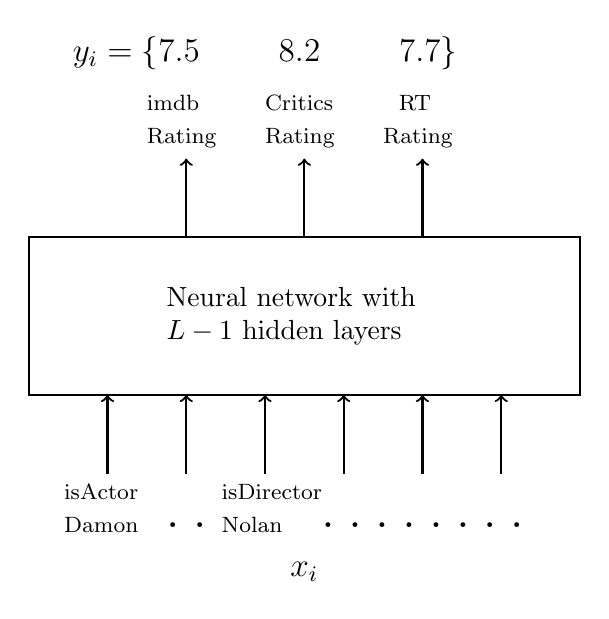
\begin{tikzpicture}[scale=1,transform shape]
	\draw[thick] (0, 0) rectangle (7, 2);
	\draw (3.5,1) node[text width=3.5cm] {Neural network with $L-1$ hidden layers};
	\draw[thick,->] (1,-1) node[below,text width=1.1cm] {\footnotesize isActor Damon} -- (1,0);
	\draw[thick,->] (2,-1) -- (2,0);
	\draw[thick,->] (3,-1) node[below,text width=1.1cm] {\footnotesize isDirector Nolan} -- (3,0);
	\draw[thick,->] (4,-1) -- (4,0);
	\draw[thick,->] (5,-1) -- (5,0);
	\draw[thick,->] (6,-1) -- (6,0);
	\draw[thick,->] (3.5,2) -- (3.5,3) node[above, text width=1cm] {\footnotesize Critics Rating};
	\draw[thick,->] (2,2) -- (2,3) node[above, text width=1cm] {\footnotesize imdb Rating};
	\draw[thick,->] (5,2) -- (5,3) node[above, text width=1cm] {\footnotesize \hspace{0.2cm}RT Rating};
	\draw (2,-1.5) node[below] {\large \textbf{. .}};
	\draw (5,-1.5) node[below] {\large \textbf{. . . . . . . .}};
	\draw (3.5,-2) node[below] {\large $x_i$};
	\draw (3,4) node[above] {\large $y_i = \left\lbrace 7.5 \hspace{1cm} 8.2 \hspace{1cm} 7.7 \right\rbrace$};
\end{tikzpicture}
}
\savestack{\nn}{% \hspace{-0.1in}
\tikzstyle{input_neuron}=[circle,draw=red!50,fill=red!10,thick,minimum size=8mm]
\tikzstyle{hidden_neuron}=[circle,draw=blue!50,fill=cyan!10,thick,minimum size=8mm]
\tikzstyle{output_neuron}=[circle,draw=green!50,fill=green!10,thick,minimum size=8mm]
\tikzstyle{bias_neuron}=[circle,draw=red!50,fill=red!10,thick,minimum size=4mm]
\tikzstyle{bias_hidden_neuron}=[circle,draw=blue!50,fill=cyan!10,thick,minimum size=4mm]
\tikzstyle{input}=[circle,draw=black!50,fill=black!20,thick,minimum size=8mm]
\begin{tikzpicture}
	\node [input_neuron] (neuron01) at (0,0) {$x_1$};
	\node [input_neuron] (neuron02) at (2,0){$x_2$};
	\node [input_neuron] (neuron03) at (4,0) {$x_n$};

	\node [bias_neuron] (neuron04) at (5.2,0.4) {};

	\node [hidden_neuron] (neuron11) at (0,2)  {};
	\node [hidden_neuron] (neuron12) at (2,2)  {};
	\node [hidden_neuron] (neuron13) at (4,2)  {};

	\node [bias_hidden_neuron] (neuron14) at (5.2,2.4) {};

	\begin{scope}
		\path[clip] (0,2) circle (4mm);
		\path[fill=blue!50] (-0.4,2) rectangle (0.4,2.4);
	\end{scope}

	\begin{scope}
		\path[clip] (2,2) circle (4mm);
		\path[fill=blue!50] (1.6,2) rectangle (2.4,2.4);
	\end{scope}

	\begin{scope}
		\path[clip] (4,2) circle (4mm);
		\path[fill=blue!50] (3.6,2) rectangle (4.4,2.4);
	\end{scope}

	\node [hidden_neuron] (neuron21) at (0,4)  {};
	\node [hidden_neuron] (neuron22) at (2,4)  {};
	\node [hidden_neuron] (neuron23) at (4,4)  {};

	\node [bias_hidden_neuron] (neuron24) at (5.2,4.4) {};

	\begin{scope}
		\path[clip] (0,4) circle (4mm);
		\path[fill=blue!50] (-0.4,4) rectangle (0.4,4.4);
	\end{scope}

	\begin{scope}
		\path[clip] (2,4) circle (4mm);
		\path[fill=blue!50] (1.6,4) rectangle (2.4,4.4);
	\end{scope}
	\begin{scope}
		\path[clip] (4,4) circle (4mm);
		\path[fill=blue!50] (3.6,4) rectangle (4.4,4.4);
	\end{scope}

	\node [output_neuron] (neuron31) at (1,6)  {};
	\node [output_neuron] (neuron32) at (3,6)  {};

	\begin{scope}
		\path[clip] (1,6) circle (4mm);
		\path[fill=green!50] (0.6,6) rectangle (1.4,6.4);
	\end{scope}

	\begin{scope}
		\path[clip] (3,6) circle (4mm);
		\path[fill=green!50] (2.6,6) rectangle (3.4,6.4);
	\end{scope}

	\draw[white,->] (neuron01) -- (neuron11) node[black,pos=.5,right]  {$W_{1}$} node[black,pos=0.8,left] {$a_{1}$};

	\draw[white,->] (neuron11) -- (neuron21) node[black,pos=.5,right] {$W_{2}$} node[black,pos=0.8,left] {$a_{2}$} node[black,pos=.2,left] {$h_{1}$};
	\draw[white,->] (neuron21) -- (neuron31) node[black,pos=.5,right] {$W_{3}$} node[black,pos=0.8,left] {$a_{3}$} node[black,pos=.2,left] {$h_{2}$};
	\draw[white,->] (neuron04) -- (neuron13) node[black,pos=0,right,above] {$b_1$};
	\draw[white,->] (neuron14) -- (neuron23) node[black,pos=0,right,above] {$b_2$};
	\draw[white,->] (neuron24) -- (neuron32) node[black,pos=0,right,above] {$b_3$};

	\draw[white,->] (neuron31) -- (1,6.5) node[black,pos=1,above] {$h_L = \hat{y} = f(x)$};

	\draw[black!20,line width=2pt,loosely dotted] (neuron01) -- (neuron02);
	\draw[black!20,line width=2pt,loosely dotted] (neuron02) -- (neuron03);
	\draw[black!20,line width=2pt,loosely dotted] (neuron11) -- (neuron12);
	\draw[black!20,line width=2pt,loosely dotted] (neuron12) -- (neuron13);
	\draw[black!20,line width=2pt,loosely dotted] (neuron21) -- (neuron22);
	\draw[black!20,line width=2pt,loosely dotted] (neuron22) -- (neuron23);
	\draw[black!20,line width=2pt,loosely dotted] (neuron31) -- (neuron32);

	\foreach \from in {neuron01,neuron02,neuron03,neuron04}
	\foreach \to in {neuron11,neuron12,neuron13}
	\draw [black!50,line width=1.5pt,->] (\from) -- (\to);

	\foreach \from in {neuron11,neuron12,neuron13,neuron14}
	\foreach \to in {neuron21,neuron22,neuron23}
	\draw [black!50,line width=1.5pt,->] (\from) -- (\to);

	\foreach \from in {neuron21,neuron22,neuron23,neuron24}
	\foreach \to in {neuron31,neuron32}
	\draw [black!50,line width=1.5pt,->] (\from) -- (\to);
\end{tikzpicture}}


\begin{frame}
  \myheading{Module 4.3: Output Functions and Loss Functions}
\end{frame}

%Slide 11
\begin{frame}
  \begin{block}{We need to answer two questions}
    \begin{itemize}
      % \justifying
      \item \alert<2>{How to choose the loss function $\mathscr{L}(\theta)$ ?} \color{black}
      \item How to compute $\nabla \theta$ which is composed of $\nabla W_1, \nabla W_2, ..., \nabla W_{L-1} \in \mathbb{R}^{n \times n}, \nabla W_L \in \mathbb{R}^{n \times k},$ \\ $\nabla b_1, \nabla b_2, ..., \nabla b_{L-1} \in \mathbb{R}^n $ and $\nabla b_L \in \mathbb{R}^k$ ?
    \end{itemize}
  \end{block}
\end{frame}

%Slide 12
\begin{frame}
  \begin{columns}
    \column{0.5\textwidth}
    \begin{overlayarea}{\textwidth}{\textheight}
      \vspace{0.3cm}
      \visible<3->{
        \makebox[\textwidth][c]{\usebox{\nnimdbexamplecontent}}
      }
    \end{overlayarea}

    \column{0.5\textwidth}
    \begin{overlayarea}{\textwidth}{\textheight}
      \begin{itemize}[<+->]
      % \justifying
        \item The choice of loss function depends on the problem at hand
        \item We will illustrate this with the help of two examples
        \item Consider our movie example again but this time we are interested in predicting ratings
        \item Here $y_i \in \mathbb{R}^3$
        \item The loss function should capture how much $\hat{y}_i$ deviates from $y_i$
        \item If $y_i \in \mathbb{R}^n$ then the squared error loss can capture this deviation
            \vspace{-0.2in}
            \begin{align*}
              \mathscr{L}(\theta) = \frac{1}{N}\sum_{i=1}^{N}\sum_{j=1}^{3}\left(\hat{y}_{ij} - y_{ij}\right)^2
            \end{align*}
      \end{itemize}
    \end{overlayarea}
  \end{columns}
\end{frame}

%Slide 13
\begin{frame}
  \begin{columns}
    \column{0.5\textwidth}
    \begin{overlayarea}{\textwidth}{\textheight}
      \makebox[\textwidth][c]{\usebox{\nncontent}}
    %   \makebox[\textwidth][c]{\usebox{\nnimdbexamplecontent}}
    \end{overlayarea}


    \column{0.5\textwidth}
    \begin{overlayarea}{\textwidth}{\textheight}
      \begin{itemize}[<+->]
      % \justifying
        \item A related question: What should the output function `$O$' be if $y_i \in \mathbb{R}$?
        \item More specifically, can it be the logistic function?
        \item No, because it restricts $\hat{y}_i$ to a value between $0$ \& $1$ but we want $\hat{y}_i \in \mathbb{R}$
        \item So, in such cases it makes sense to have `$O$' as identity function
            \begin{align*}
              f(x) & = h_{L} = O(a_{L})             \\
                 & = a_{L} = W_{L}h_{L-1} + b_{L}
            \end{align*}

        \item $\hat{y}_i = f(x_i)$ is no longer bounded between 0 and 1
      \end{itemize}
    \end{overlayarea}
  \end{columns}
\end{frame}

\begin{frame}[b]
    \visible<1-2>{\tiny Intentionally left blank}
\end{frame}

%Slide 14
\begin{frame}
  \begin{columns}
    \column{0.5\textwidth}
    \begin{overlayarea}{\textwidth}{\textheight}
      \vspace{0.3cm}
      \makebox[\textwidth][c]{\usebox{\nnfruitclassexamplecontent}}
    \end{overlayarea}

    \column{0.5\textwidth}
    \begin{overlayarea}{\textwidth}{\textheight}
      \begin{itemize}[<+->]
      % \justifying
        \item Now let us consider another problem for which a different loss function would be appropriate
        \item Suppose we want to classify an image into $1$ of $k$ classes
        \item Here again we could use the squared error loss to capture the deviation
        \item But can you think of a better function?
      \end{itemize}
    \end{overlayarea}
  \end{columns}
\end{frame}

%Slide 15
\begin{frame}
  \begin{columns}
    \column{0.5\textwidth}
    \begin{overlayarea}{\textwidth}{\textheight}
      \only<1-2>{
        \vspace{0.3cm}
        \makebox[\textwidth][c]{\usebox{\nnfruitclassexamplecontent}}
      }
      \only<3->{
        \makebox[\textwidth][c]{\usebox{\nncontent}}
      }
    \end{overlayarea}

    \column{0.5\textwidth}
    \begin{overlayarea}{\textwidth}{\textheight}
      \begin{itemize}
        % \justifying
        \item<1-> Notice that $y$ is a probability distribution
        \item<2-> Therefore we should also ensure that $\hat{y}$ is a probability distribution
        \item<3-> What choice of the output activation `$O$' will ensure this ?
            \vspace{-0.1in}
            \begin{align*}
              a_{L}               & = W_{L}h_{L-1} + b_{L}                                            \\
              \visible<4->{f(x)_j & = O(a_{L})_j = \frac{e^{a_{L, j}}}{\sum_{j'=1}^{k} e^{a_{L,j'}}}}
            \end{align*}
            % \vspace{-0.1in}
            \visible<4->{$O(a_{L})_j$ is the $j^{th}$ element of $\hat{y}$\\ $a_{L,j}$ is the $j^{th}$ element of the vector $a_{L}$.}
        \item<5-> This function is called the \textit{softmax} function
      \end{itemize}
    \end{overlayarea}
  \end{columns}
\end{frame}

%Slide 16
\begin{frame}
  \begin{columns}
    \column{0.5\textwidth}
    \begin{overlayarea}{\textwidth}{\textheight}
      \vspace{0.3cm}
      \makebox[\textwidth][c]{\usebox{\nnfruitclassexamplecontent}}
    \end{overlayarea}

    \column{0.5\textwidth}
    \begin{overlayarea}{\textwidth}{\textheight}
      \begin{itemize}
        % \justifying
        \item<1-> Now that we have ensured that both $y$ \& $\hat{y}$ are probability distributions can you think of a function which captures the difference between them?
        \item<2-> Cross-entropy \begin{equation*}
              \mathscr{L}(\theta) = - \sum_{c=1}^{k} y_c \log \hat{y}_c
            \end{equation*}
        \item<3-> Notice that \begin{align*}
              y_c                 & = 1 \hspace{0.5cm} \text{if $c=\ell$ (the true class label)} \\
                        & = 0 \hspace{0.5cm} \text{otherwise}                          \\
              \mathscr{L}(\theta) & = - \log \hat{y}_{\ell}
            \end{align*}
      \end{itemize}
    \end{overlayarea}
  \end{columns}
\end{frame}

%Slide 17
\begin{frame}
  \begin{columns}
    \column{0.35\textwidth}
    \begin{overlayarea}{\textwidth}{\textheight}
      \vspace{0.3cm}
      \makebox[\textwidth][c]{\usebox{\nncontent}}
      % \makebox[\textwidth][c]{\usebox{\nnfruitclassexamplecontent}}
    \end{overlayarea}

    \column{0.65\textwidth}
    \begin{overlayarea}{\textwidth}{\textheight}
      \begin{itemize}[<+->]
      % \justifying
        \item So, for classification problem (where you have to choose $1$ of $K$ classes), we use the following objective function
          \begin{align*}
                        \underset{\theta}{\text{minimize}} ~~~~~~\mathscr{L}_\theta &= -\log \hat{y}_{\ell} \\ %\{- \log \hat{y}_{\ell}\}$ \\ 
              \text{or}~~~~~~\underset{\theta}{\text{maximize}} ~~ -\mathscr{L}_\theta &=  \log \hat{y}_{\ell}    %\{- \log \hat{y}_{\ell}\}$ \\ 
          \end{align*}
          % \hspace{2cm}
          % \hspace{2cm} 
          %     or $\max \log \hat{y}_{\ell}$
        \item But wait! \\
            Is $\hat{y}_\ell$ a function of $\theta=[W_1,W_2,.,W_L,b_1,b_2,.,b_L]$?
        \item Yes, it is indeed a function of $\theta$
          \begin{center}
            $ \hat y_\ell = [O(W^{3}g(W^{2}g(W^{1}x+b_{1})+b_{2})+b_{3})]_\ell $
          \end{center}
        \item What does $\hat{y}_\ell$ encode? 
        \item It is the probability that $x$ belongs to the $\ell^{th}$ class (bring it as close to $1$).
        \item $\log \hat{y}_\ell$ is called the \textit{log-likelihood} of the data.
      \end{itemize}
    \end{overlayarea}
  \end{columns}
\end{frame}

%Slide 18
\begin{frame}
  \begin{overlayarea}{\textwidth}{\textheight}
    \begin{center}
      \begin{table}[]
        \centering
        \label{my-label}
        \renewcommand{\arraystretch}{2}
        \begin{tabular}{c|c|c|}
          \cline{2-3}
                              & \multicolumn{2}{        c|}{\textbf{Outputs}} \\ \cline{2-3} 
                              & Real Values             & Probabilities     \\ \hline
          \multicolumn{1}{|c|}{Output Activation} & \visible<2->{Linear}       & \alert<7>{\visible<3->{Softmax}}\\ \hline
          \multicolumn{1}{|c|}{Loss Function}     & \visible<4->{Squared Error}& \alert<7>{\visible<5->{Cross Entropy}}   \\ \hline
        \end{tabular}
        \renewcommand{\arraystretch}{1}
      \end{table}
    \end{center}

    \begin{itemize}
      % \justifying
      \item<6-> Of course, there could be other loss functions depending on the problem at hand but the two loss functions that we just saw are encountered very often
      \item<7-> For the rest of this lecture we will focus on the case where the output activation is a softmax function and the loss function is cross entropy
    \end{itemize}
  \end{overlayarea}
\end{frame}